\appendix
\chapter{Anlagen}
\section{Well-Known-Binary Format (WKB)}
\label{sec:appendix:wkb}
Das \textit{Well-Known-Binary} Format ist die binäre Repräsentation eines geometrischen Objekts des \textit{Simple Feature Models}.
Das Simple Feature Model ist eine Untermenge des ISO 19107 Standards, welcher die geometrischen Eigenschaften von Geoobjekten spezifiziert. Ausgehend von einer allgemeinen Oberklasse können geometrische Primitive, wie z.B. ein Punkt, oder komplexe geometrische Objekte, wie z.B. Flächen oder Sammlungen von Objekten, beschrieben werden. (vgl. \cite{Bill2010}:358ff.). Die verfügbaren Klassen werden in Abbildung \ref{fig:bill_sfm} aufgezeigt.
\begin{figure}[!htb]
  \centering
   \fbox{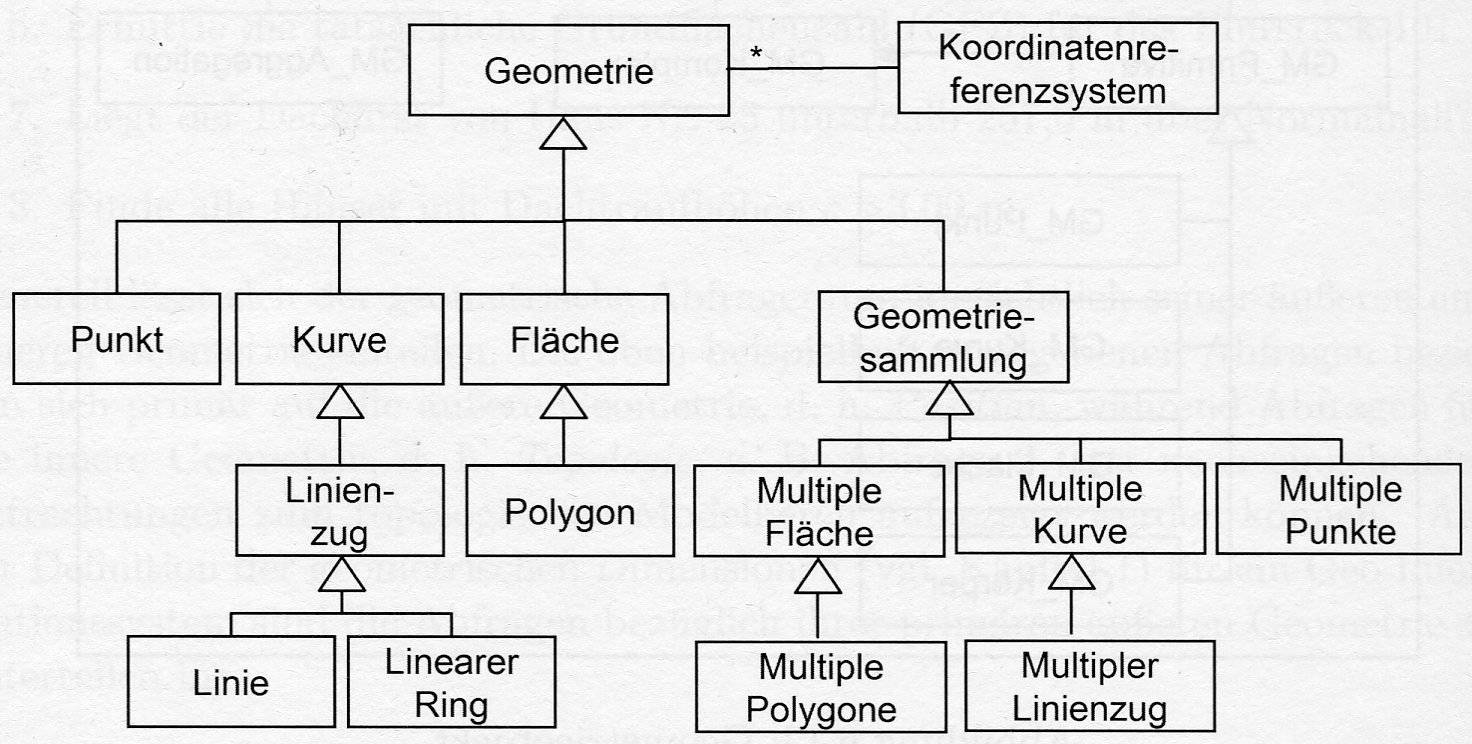
\includegraphics[width=1\textwidth]{gfx/bill_sfm001.jpg}}
   \caption{Geometrien im Simple Feature Model \protect\cite{Bill2010}:360}
   \label{fig:bill_sfm}
\end{figure}

Das WKB Format wird beispielsweise innerhalb der PostgreSQL Erweiterung PostGIS\footnote{http://postgis.net} genutzt, um geometrische Objekte in einer Datenbank abzulegen.
Analog dazu existiert das \textit{Well-Known-Text} Format, welches die textuelle Repräsentation geometrische Objekte des Simple Feature Models spezifiziert.

\subsubsection{Beispiel für das WKB und das WKT Format}
Ein Punkt mit den Koordinaten \texttt{13.439561 Ost} sowie \texttt{52.54002 Nord} entspricht der WKT Repräsentation\\\\
\texttt{SRID=4326;POINT(13.439561 52.54002)}\\\\
und der WKB Repräsentation\\\\
\texttt{0101000020E6100000B131AF230EE12A40CC9717601F454A40}\\\\
Der Wert \texttt{SRID} beinhaltet die ID des zu verwendenden Koordinatenreferenzsystems.
Die ID \texttt{4326} entspricht dem häufig verwendeten Referenzsystem \texttt{WGS84}\footnote{http://spatialreference.org/ref/epsg/4326/}.  

\section{GeoJSON}
\label{sec:appendix:geojson}
GeoJSON\footnote{http://geojson.org} ist ein Format zur Repräsentation von geometrischen Objekten im JSON Format.
Es verwendet ein ähnliches hierarchisches Klassenmodell. (vgl. \cite{WEB:GEOJSON:Spec:2008}).

\subsubsection{Beispiel für das GeoJSON Format}
Ein Punkt mit den Koordinaten \texttt{13.439561 Ost} sowie \texttt{52.54002 Nord} entspricht der GeoJSON Repräsentation
\begin{lstlisting}
  {
    "type": "Point",
    "coordinates": [
        13.439561,
        52.54002
    ]
}
\end{lstlisting}

\section{OpenStreetMap Datenformat}
\label{sec:appendix:osm:data}
OpenStreetMap bietet seine Daten zum Download in einer Datei, \textit{planet.osm}\footnote{http://planet.openstreetmap.org/}, an. Diese Datei im XML-Format enthält den kompletten Datenbestand des OpenStreetMap Projekts. 
Da diese Datei sehr groß ist (gepackt ca. 50GB) bieten andere Dienstleister wie zum Beispiel die Geofabrik GmbH Karlsruhe\footnote{http://www.geofabrik.de} auch kleinere Bereiche des Datenbestandes, zum Beispiel nur Deutschland, an.
Zur Speicherung der Daten werden die Elemente \textit{Nodes}, \textit{Ways} und \textit{Relations} verwendet. (vgl. \cite{WEB:OSM:Primitives:2015})
\begin{compactitem}
  \item \textbf{Nodes}, ein geometrischer Punkt, welcher durch geographische Breite und Länge bestimmt ist
  \item \textbf{Ways}, ein Linienzug zwischen mehreren Punkten. Hiermit werden zum Beispiel Straßen, Flüsse und vieles mehr modelliert
  \item \textbf{Relations}, eine logische Gruppierung mehrerer \textit{Nodes}, \textit{Ways} oder auch \textit{Relations}. Die Mitglieder einer Relation haben einen Bezug zueinander, zum Beispiel ein Wald mit seinen Lichtungen oder ein Bahnhof. 
\end{compactitem}
Alle Elemente können wiederum durch \textit{Tags} mit Eigenschaften versehen werden.

\subsubsection{Beispiel eines Nodes}
\begin{lstlisting}
<node id="3637807236" visible="true" version="1" changeset="32456135" timestamp="2015-07-06T19:04:03Z" user="bigbug21" uid="15748" lat="50.5379840" lon="12.1402231"/>
\end{lstlisting}

\subsubsection{Beispiel eines Ways}
\begin{lstlisting}
  <way id="358952758" visible="true" version="1" changeset="32456135" timestamp="2015-07-06T19:04:13Z" user="bigbug21"  uid="15748">
  <nd ref="3637807236"/>
  <nd ref="3637807232"/>
  <nd ref="3637807230"/>
  <nd ref="3637806843"/>
  <nd ref="3637806841"/>
  <tag k="public_transport" v="platform"/>
  <tag k="railway" v="platform"/>
  <tag k="train" v="yes"/>
 </way>
\end{lstlisting}

\subsubsection{Beispiel einer Relation}
\begin{lstlisting}
<relation id="2303826" visible="true" version="9" changeset="34783224" timestamp="2015-10-21T17:05:38Z" user="Kakaner" uid="1851521">
  <member type="way" ref="166800600" role=""/>
  <member type="way" ref="166800590" role=""/>
  <member type="way" ref="166800593" role=""/>
  <member type="way" ref="166800357" role=""/>
  <member type="way" ref="376274301" role=""/>
  <member type="way" ref="166800198" role=""/>
  <member type="way" ref="165821978" role=""/>
  <member type="way" ref="165821752" role=""/>
  <member type="way" ref="165741930" role=""/>
  <member type="way" ref="165741583" role=""/>
  <member type="way" ref="165479804" role=""/>
  <member type="way" ref="165479800" role=""/>
  <member type="way" ref="165479712" role=""/>
  <member type="way" ref="165409360" role=""/>
  <member type="way" ref="165408947" role=""/>
  <member type="way" ref="264419428" role=""/>
  <member type="way" ref="165022595" role=""/>
  <member type="way" ref="165022069" role=""/>
  <member type="way" ref="164988309" role=""/>
  <member type="way" ref="164987948" role=""/>
  <member type="way" ref="159213270" role=""/>
  <member type="way" ref="264419420" role=""/>
  <member type="way" ref="376165609" role=""/>
  <member type="way" ref="158208266" role=""/>
  <member type="way" ref="159211943" role=""/>
  <member type="way" ref="264419427" role=""/>
  <member type="way" ref="356950454" role=""/>
  <member type="way" ref="158207942" role=""/>
  <member type="way" ref="158206932" role=""/>
  <member type="way" ref="250106659" role=""/>
  <member type="way" ref="250106648" role=""/>
  <member type="way" ref="254270906" role=""/>
  <member type="way" ref="158511899" role=""/>
  <member type="way" ref="158511802" role=""/>
  <member type="way" ref="159211993" role=""/>
  <tag k="operator" v="Vogtlandbahn"/>
  <tag k="public_transport:version" v="2"/>
  <tag k="ref" v="VB2"/>
  <tag k="route" v="train"/>
  <tag k="type" v="route"/>
 </relation>
\end{lstlisting}

\section{Beispiel einer Straße in OpenStreetMap}
\label{sec:appenix:osm:streets}